\documentclass[11pt, addpoints, answers]{exam}

\usepackage[utf8]{inputenc}
\usepackage[T1]{fontenc}
\usepackage[margin  = 1in]{geometry}
\usepackage{amsmath, amscd, amssymb, amsthm, verbatim}
\usepackage{mathabx}
\usepackage{setspace}
\usepackage{float}
\usepackage{color}
\usepackage{graphicx}   
\usepackage[colorlinks=true]{hyperref}
\usepackage{tikz}

\usetikzlibrary{shapes,arrows}
%%%<
\usepackage{verbatim}
%%%>
\usetikzlibrary{automata,arrows,positioning,calc}

\usetikzlibrary{trees}

\shadedsolutions
\definecolor{SolutionColor}{RGB}{214,240,234}

% \usepackage{xcolor}
\usepackage{listings}

\lstset{language=R,
    basicstyle=\small\ttfamily,
    stringstyle=\color{black},
    otherkeywords={0,1,2,3,4,5,6,7,8,9},
    morekeywords={TRUE,FALSE},
    deletekeywords={data,frame,length,as,character},
    keywordstyle=\color{blue}
}

\newcommand{\bbC}{{\mathbb C}}
\newcommand{\R}{\mathbb{R}}            % real numbers
\newcommand{\bbR}{{\mathbb R}}
\newcommand{\Z}{\mathbb{Z}}            % integers
\newcommand{\bbZ}{{\mathbb Z}}
\newcommand{\bx}{\mathbf x}            % boldface x
\newcommand{\by}{\mathbf y}            % boldface y
\newcommand{\bz}{\mathbf z}            % boldface z
\newcommand{\bn}{\mathbf n}            % boldface n
\newcommand{\br}{\mathbf r}            % boldface r
\newcommand{\bc}{\mathbf c}            % boldface c
\newcommand{\be}{\mathbf e}            % boldface e
\newcommand{\bE}{\mathbb E}            % blackboard E
\newcommand{\bP}{\mathbb P}            % blackboard P

\newcommand{\ve}{\varepsilon}          % varepsilon
\newcommand{\avg}[1]{\left< #1 \right>} % for average
%\renewcommand{\vec}[1]{\mathbf{#1}} % bold vectors
\newcommand{\grad}{\nabla }
\newcommand{\lb}{\langle }
\newcommand{\rb}{\rangle }

\def\Bin{\operatorname{Bin}}
\def\Var{\operatorname{Var}}
\def\Geom{\operatorname{Geom}}
\def\Pois{\operatorname{Pois}}
\def\Exp{\operatorname{Exp}}
\def\Weibull{\operatorname{Weibull}}
\newcommand{\Ber}{\operatorname{Ber}}
\def\Unif{\operatorname{Unif}}
\def\No{\operatorname{N}}
\newcommand{\E}{\mathbb E}            % blackboard E
\def\th{\theta }            % theta shortcut
\def\V{\operatorname{Var}}
\def\Var{\operatorname{Var}}
\def\Cov{\operatorname{Cov}}
\def\Corr{\operatorname{Corr}}
\newcommand{\epsi}{\varepsilon}            % epsilon shortcut

\providecommand{\norm}[1]{\left\lVert#1\right\rVert} %norm
\providecommand{\abs}[1]{\left \lvert#1\right \rvert} %absolute value

\DeclareMathOperator{\lcm}{lcm}
\newcommand{\ds}{\displaystyle}	% displaystyle shortcut

% Distributions.
% \newcommand*{\UnifDist}{\mathsf{Unif}}
% \newcommand*{\ExpDist}{\mathsf{Exp}}
% \newcommand*{\DepExpDist}{\mathsf{DepExp}}
% \newcommand*{\GammaDist}{\mathsf{Gamma}}
% \newcommand*{\LognormalDist}{\mathsf{LogNorm}}
% \newcommand*{\WeibullDist}{\mathsf{Weib}}
% \newcommand*{\ParetoDist}{\mathsf{Par}}
% \newcommand*{\NormalDist}{\mathsf{Normal}}

% \newcommand*{\GeometricDist}{\mathsf{Geom}}
% \newcommand*{\NegBinomialDist}{\mathsf{NegBin}}
% \newcommand*{\BinomialDist}{\mathsf{Bin}}
% \newcommand*{\PoissonDist}{\mathsf{Poisson}}
\newcommand*{\Prob}{\mathbb{P}}
% \newcommand*{\Cov}{\mathsf{Cov}}


\def\semester{2023-2024}
\def\course{Modèle de Durée}
\def\title{\MakeUppercase{Examen final}}
\def\name{Pierre-O Goffard}
%\def\name{Professor Wildman}

\setlength\parindent{0pt}

\cellwidth{.35in} %sets the minimum width of the blank cells to length
\gradetablestretch{2.5}

%\bracketedpoints
%\pointsinmargin
%\pointsinrightmargin

\begin{document}


\runningheader{\course  \vspace*{.25in}}{}{\title \vspace*{.25in}}
%\runningheadrule
\runningfooter{}{Page \thepage\ of \numpages}{}

% \firstpageheader{Name:\enspace\hbox to 2.5in{\hrulefill}\\  \vspace*{2em} Section: (circle one) TR: 3-3:50 \textbar\, TR: 5-5:50 \textbar\,  TR: 6-6:50(Xu) \textbar\,  TR: 6-6:50 }{}{Perm \#: \enspace\hbox to 1.5in{\hrulefill}\\ \vspace*{2em} Score:\enspace\hbox to .6in{\hrulefill} $/$\numpoints}
\extraheadheight{.25in}

\hrulefill

\vspace*{1em}

% Heading
{\center \textsc{\Large\title}\\
	\vspace*{1em}
	\course -- \semester\\
	Pierre-O Goffard\\
}
\vspace*{1em}

\hrulefill

\vspace*{2em}

\noindent {\bf\em Instructions:} On éteint et on range son téléphone.
\begin{itemize}
	\item La calculatrice et les appareils éléctroniques ne sont pas autorisés.
	\item Vous devez justifier vos réponses de manière claire et concise.
	\item Vous devez écrire de la manière la plus lisible possible. Souligner ou encadrer votre réponse finale.
	\item \underline{Document autorisé:} Une feuille manuscrite recto-verso

\end{itemize}


\begin{center}
	\gradetable[h]
\end{center}

\smallskip

\begin{questions}
\question[4] Nous souhaitons calibrer sur nos données un modèle exponentiel $\text{Exp}(\beta)$ de densité
$$
f(t) = \frac{e^{-t/\beta}}{\beta}\mathbb{I}_{(0,\infty)}(t),
$$
avec $\beta>0$. 

Nous disposons d'un échantillon de taille $n$. Nos données sont à la fois tronquées à gauche, avec un niveau de troncature $c>0$ pour toutes les observations et censurées à droites, avec un niveau de censure $c_1, \ldots, c_n$, différent pour chaque observation tels que $c_i >c$ pour tout $i=1,\ldots, n$. 

Donner l'estimateur du maximum de vraisemblance pour le paramètre $\beta$. Il faut rappeler les notations pour les données censurées et détailler les étapes de calcul menant à l'expression de l'estimateur.
\begin{solution}
Les données sont notée 
$$
\mathcal{D} = (x_i,\delta_i)_{i = 1,\ldots, n} = (t_i\land c_i,\mathbb{I}_{t_i\leq c_i})_{i = 1,\ldots, n},
$$
où $t_i$ sont les observations non censurées. Ces observations non-censurées sont tronquées à gauche au niveau $c$, leur densité est donnée par 
$$
f_{(c,\infty)}(t) = \frac{e^{-(t-c)/\beta}}{\beta}\mathbb{I}_{(c,\infty)}(t),
$$
leur fonction de survie par 
$$
S_{(c,\infty)}(t) = \begin{cases}
1,&\text{ }si t\leq c,\\
e^{-(t-c)/\beta},& t>c.
\end{cases}
$$
et leur fonction de hasard est donnée par
$$
h_{(c,\infty)}(t) = \frac{1}{\beta}\mathbb{I}_{(c,\infty)}(t).
$$
La log-vraisemblance des observation est donnée par 
$$
l(\mathcal{D};\beta) = \frac{1}{\beta}\sum \delta_i - \frac{1}{\beta^2}\sum (x_i - c)
$$
L'équation 
$$
\frac{\partial }{\partial \beta}l(\mathcal{D};\beta) = 0,
$$
équivaut à 
$$
\hat{\beta} = \frac{\sum(x_i - c)}{\sum\delta_i}.
$$
On peut vérifier que 
$$
\frac{\partial^2 }{\partial \beta^2}l(\mathcal{D};\beta)\Big\rvert_{\beta = \hat{\beta}}  < 0
$$

\end{solution} 
\question Nous avons des données de mortalité pour la Belgique pendant l'année 2000 pour des personnes agées de 30 à 105 ans, voir le Tableau \ref{tab:death_count_belgium}.
\begin{table}[!ht]
\centering
\begin{tabular}{rrrr}
Age & Year & $E_x^c$ &$ D_x$ \\ 
  \hline
30 & 2000 & 146944 & 119 \\ 
  31 & 2000 & 147252 & 135 \\ 
  32 & 2000 & 148805 & 132 \\ 
  33 & 2000 & 152792 & 160 \\ 
  34 & 2000 & 157925 & 161 \\ 
  35 & 2000 & 163324 & 155 \\ 
   \hline
\end{tabular}
\caption{Nombre de décès et expositions centrales pour la Belgique pendant l'année 2000.}
\label{tab:death_count_belgium}
\end{table}
\begin{parts}
\part[1] Nous allons estimer les taux de mortalité via le modèle de Poisson. Rappeler les hypothèses du modèle et l'expression de l'estimateur des taux de mortalités.
\begin{solution}
Dans le cadre du modèle de Poisson, on suppose que 
$$
D_x\sim\text{Pois}()\mu_x\cdot E_x^c),
$$
où $D_x$ est le nombre de décès parmi les individus d'âge $x$, $E_x^c$ est l'exposition centrale pour les individus d'âge $x$ et $\mu_x$ est le taux de mortalité pour les individus d'âge $x$. Les taux de mortalités sont estimés par 
$$
\hat{\mu}_x = \frac{D_x}{E_x^c}.
$$
\end{solution}
\part[1] La Figure \ref{fig:mux_raw} montre les taux de mortalités estimés en fonction de l'âge.
\begin{figure}[!ht]
\centering
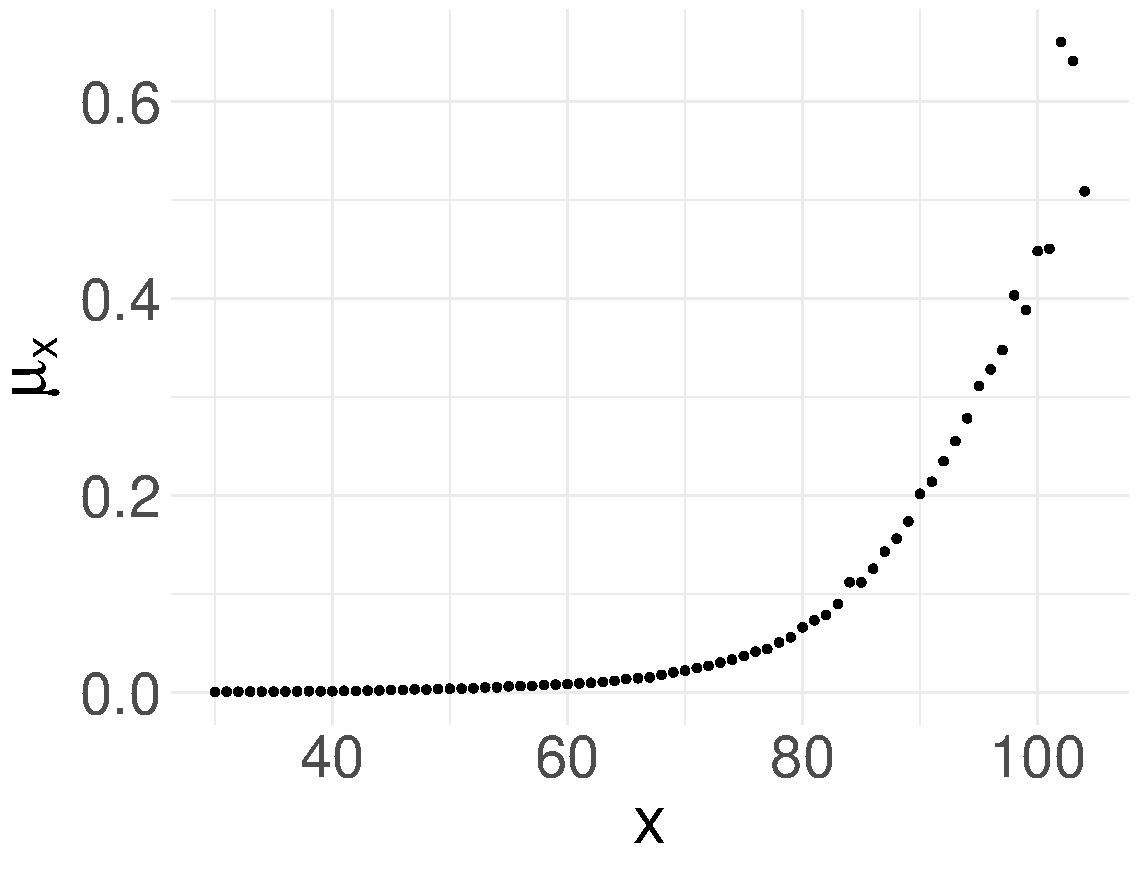
\includegraphics[width = 0.4\textwidth]{figures/mux_raw.pdf}
\caption{Taux de mortalité en fonction de l'âge.}
\label{fig:mux_raw}
\end{figure}
Nous allons ajuster le modèle suivant:
\begin{equation}\label{eq:modele_weibull}
\mu_x = \left(\frac \alpha\beta\right) \cdot \left(\frac x\beta\right)^{\alpha - 1},
\end{equation}
sur les taux estimés de la Figure \ref{tab:death_count_belgium}. De quel type de procédure s'agit-il? Quel est l'intérêt d'une telle procédure?
\begin{solution}
Il s'agit d'une procédure de lissage paramétrique. Elle permet de remplacer les taux de mortalités aux grands âge peu fiable du fait de la faible exposition. 
\end{solution}
\part[1] La Figure \ref{fig:log_mux_raw} montre le logarithme des taux de mortalités en fonction du log de l'âge.

\begin{figure}[!ht]
\centering
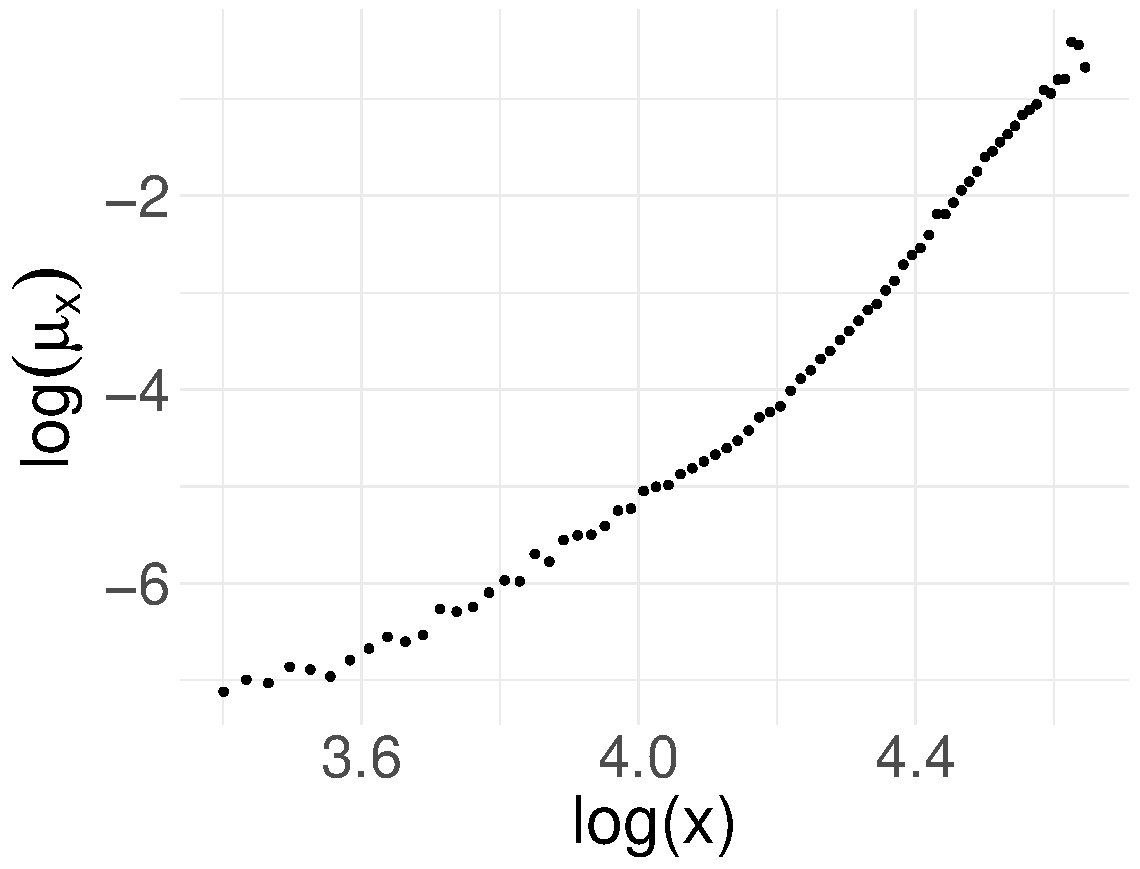
\includegraphics[width = 0.35\textwidth]{figures/log_mux_raw.pdf}
\caption{Log des taux de mortalité en fonction du log de l'âge.}
\label{fig:log_mux_raw}
\end{figure}
En quoi ce graphique conforte le choix du modèle de la question b)?
\begin{solution}
En prenant le log dans l'équation \eqref{eq:modele_weibull}, il vient
$$
\log(\mu_x) = \log(\alpha)-\alpha\log(\beta) +  (\alpha - 1)\log(x).
$$
Notre modèle de lissage suppose donc un lien linéaire entre le log des taux de mortalité et le log de l'âge. On constate peu ou proue ce lien sur la Figure \ref{fig:log_mux_raw}.
\end{solution}
\part[1] Les données de mortalité du Tableau \ref{tab:death_count_belgium} sont stockées dans un data frame $R$, appelé \texttt{df$\_$Bel}. Nous faisons tourné le programme suivant:
\begin{lstlisting}
df_Bel_V1 <- df_Bel %>% 
mutate(mux = Dx / ExC, logx = log(Age), logmux = log(mux))

res <- lm(logmux ~ logx, data = df_Bel_V1)
\end{lstlisting}
Le contenu de l'objet \texttt{res} est donné sur la Figure \ref{fig:lm_scren_shot}.
\begin{figure}[!ht]
\centering
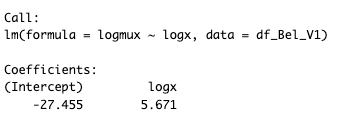
\includegraphics[width = 0.6\textwidth]{figures/lm_screen_shot.png}
\caption{Contenu de l'objet \texttt{res}.}
\label{fig:lm_scren_shot}
\end{figure}

Peut-on déduire la valeur de $\alpha$ et $\beta$ de la sortie R de la Figure \ref{fig:lm_scren_shot}? Expliquer.
\begin{solution}
En notant $a = -27.455$ et $b = 5.671$, on identifie 
$$
\begin{cases}
a = \log(\alpha) - \alpha\log(\beta)
b = \alpha - 1\\
\end{cases}
$$
ce qui équivaut à 
$$
\begin{cases}
\alpha = b +1 \\
\beta = \exp\left(\frac{\log(b+1) - a}{b+1}\right)
\end{cases}
$$
\end{solution}
\part[2] Les taux de mortalités issus du modèle de la question b) sont donnés sur la Figure \ref{fig:mux_raw_VS_smoothed}.
\begin{figure}[!ht]
\centering
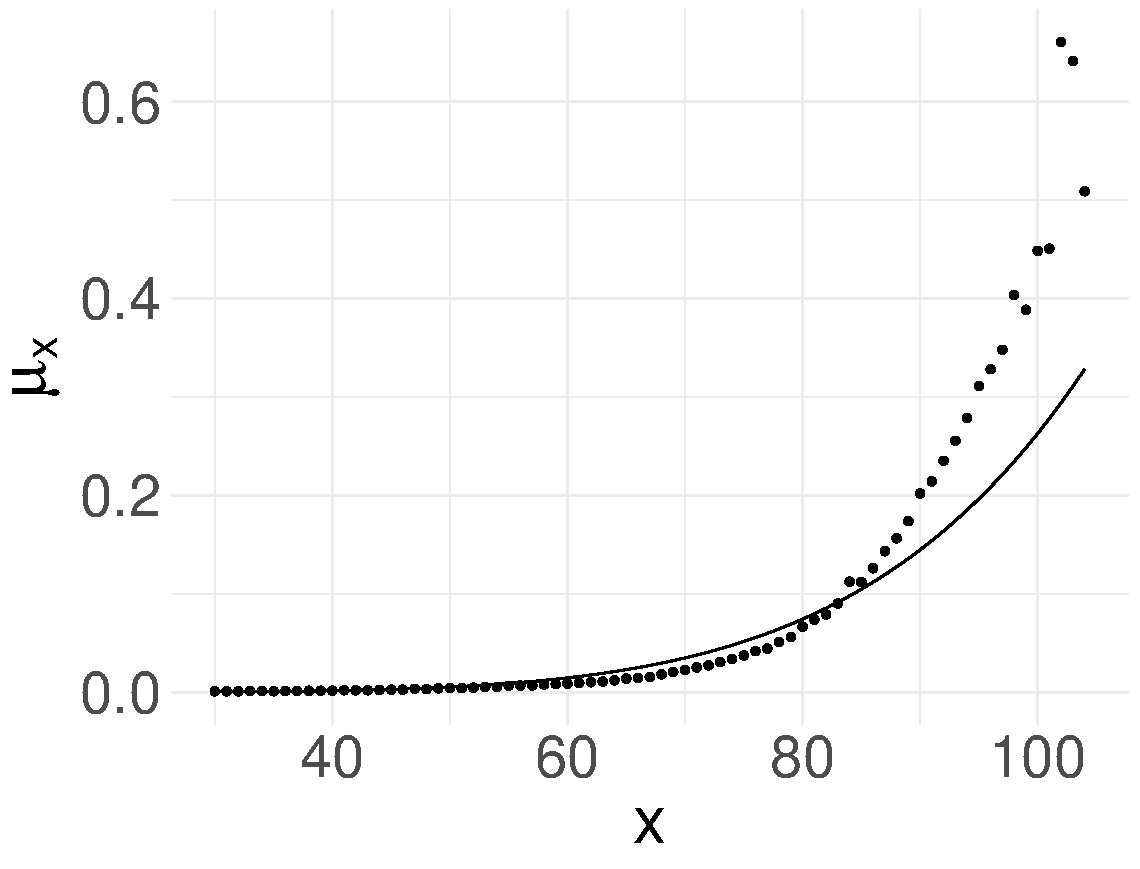
\includegraphics[width = 0.4\textwidth]{figures/mux_raw_VS_smoothed}
\caption{Taux de mortalité estimé (points) et ajustés avec le modèle de la question b) (trait plein).}
\label{fig:mux_raw_VS_smoothed}
\end{figure}

Que pensez vous de cet ajustement ? Comment pourrait-on l'améliorer? On pourra s'appuyer sur les Figures \ref{fig:log_mux_raw} et \ref{fig:mux_raw_VS_smoothed} pour répondre. Pour information $\exp(4)\approx 54.6$.
\begin{solution}
Cet ajustement est assez peu satisfaisant car il conduit à une sur-estimation des taux de mortalités aux jeunes âges et une sur-estimation au âges plus avancés. On remarque sur la figure \ref{fig:log_mux_raw} une cassure pour $log(x) = 4$ avec potentiellement deux tendances linéaires distinctes pour les plages $x\in(30, e^4)$ et $x\in(e^4, 105)$. Une solution serait d'ajuster le modèle séparément sur ces deux plages ou bien seulement remplacer les taux de mortalités à partir de $x > e^4$ par ceux du modèle calibré sur la plage $x\in(e^4,105)$.
\end{solution}
\part[2] En admettant que l'on ait été en mesure de déterminer $\alpha$ et $\beta$, nous les stockons dans les variables \texttt{alpha} et \texttt{beta}. Cela nous permet de calculer les taux de mortalités ajustés par le modèle de la question b). On fait tourner le programme R suivant:
\begin{lstlisting}
df_Bel_smooth <- df_Bel_V1 %>% 
mutate( mux_smooth = ( alpha / beta) * (Age / beta)^(alpha - 1))

res_binom_test <- binom.test(
sum(df_Bel_smooth$mux > df_Bel_smooth$mux_smooth), 
nrow(df_Bel_smooth), 
p=0.5)
\end{lstlisting}
Le contenu de l'objet \texttt{res$\_$binom$\_$test} est donné par la Figure \ref{fig:binom_test_screen_shot}.
\begin{figure}[!ht]
\centering
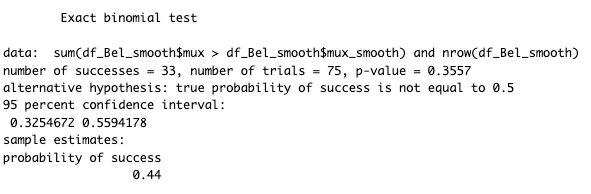
\includegraphics[width = 0.9\textwidth]{figures/binom_test_screen_shot.png}
\caption{contenu de l'objet \texttt{res$\_$binom$\_$test}.}
\label{fig:binom_test_screen_shot}
\end{figure}

De quelle procédure s'agit-il et quel est son intérêt? Quelle interprétation faites-vous du résultat?
\begin{solution}
Il s'agit d'un test des signe permettant de valider la méthode de lissage en vérifiant que la procédure de lissage ne sous ou sur-estime pas systématiquement les taux de mortalité brut. Nous observon que la p-valeur ne permet de rejeter $H_0$ suivant laquelle la probabilité de sur ou de sous-estimation est égale à 0.5. Le test des signe est un succès, on pouvait s'y attendre puisque qu'on sur estime pour les jeunes âges et sous-estime pour les grnds âges. Un test des run pourrait être effectué en complément, il conduirait à indiqué la présence de sur-estimation ou de sous-estimation successive qui démontrerait que la méthode de lissage n'est pas optimale. 
\end{solution}
\end{parts}
\question Les données contiennent des mesures effectuées sur des patients atteints de mélanome. Chaque patient a subi une ablation de la tumeur par chirurgie au Département de Chirurgie Plastique de l’Hôpital Universitaire d’Odense, au Danemark, pendant la période de 1962 à 1977. Un extrait des données est fourni par le Tableau \ref{tab:extrait_melanome}.
\begin{table}[!ht]
\centering
\begin{tabular}{rrrrrrr}
  \hline
time & status & sex & age & year & thickness & ulcer \\ 
  \hline
10 & 3 & 1 & 76 & 1972 & 6.76 & 1 \\ 
  30 & 3 & 1 & 56 & 1968 & 0.65 & 0 \\ 
  35 & 2 & 1 & 41 & 1977 & 1.34 & 0 \\ 
  99 & 3 & 0 & 71 & 1968 & 2.90 & 0 \\ 
  185 & 1 & 1 & 52 & 1965 & 12.08 & 1 \\ 
  204 & 1 & 1 & 28 & 1971 & 4.84 & 1 \\ 
   \hline
\end{tabular}
\caption{Extrait des données de patients ayant été opéré pour un mélanome}
\label{tab:extrait_melanome}
\end{table}

Voici une courte description des variables:
\begin{itemize}
  \item \texttt{time}: Temps de survie depuis l'opération (nombre de jours) 
  \item \texttt{status}: Variable catégorielle indiquant si le patient est mort à cause du mélanome (1), a survécu jusqu' à la fin de l'étude (2), est mort d'une cause autre que le mélanome (3). 
  \item \texttt{sex}: Genre du patient (0 = Femme et 1 = Homme) 
  \item \texttt{age}: Age du patient en année
  \item \texttt{year}: Année de l'opération 
  \item \texttt{thickness}: Epaisseur de la tumeur en millimètres
  \item \texttt{ulcer}: Présence (1) ou Absence (0) d'un ulcère sur la tumeur
\end{itemize}

Nous allons considérer la survie des patients sans distinguer la cause du décès entrainant le recodage suivant de la variable \texttt{status}:
\begin{lstlisting}
melanoma <- melanoma %>%
  mutate(status_os = if_else(status == 2, 0, 1))
\end{lstlisting}
\begin{parts}
\part[2] Nous nous intéressons d'abord à l'impact variable \texttt{ulcer} sur la survie des patients. Nous commençons par faire tourner le code suivant: 
\begin{lstlisting}
fit <- survfit(Surv(time, status_os) ~ ulcer, data = melanoma)
ggsurvplot(fit, pval = FALSE, conf.int = TRUE, linetype = "strata",
 ggtheme = theme_minimal())
\end{lstlisting}
Le résultat est donné sur la Figure \ref{fig:KM_plot}.
\begin{figure}[!ht]
\centering
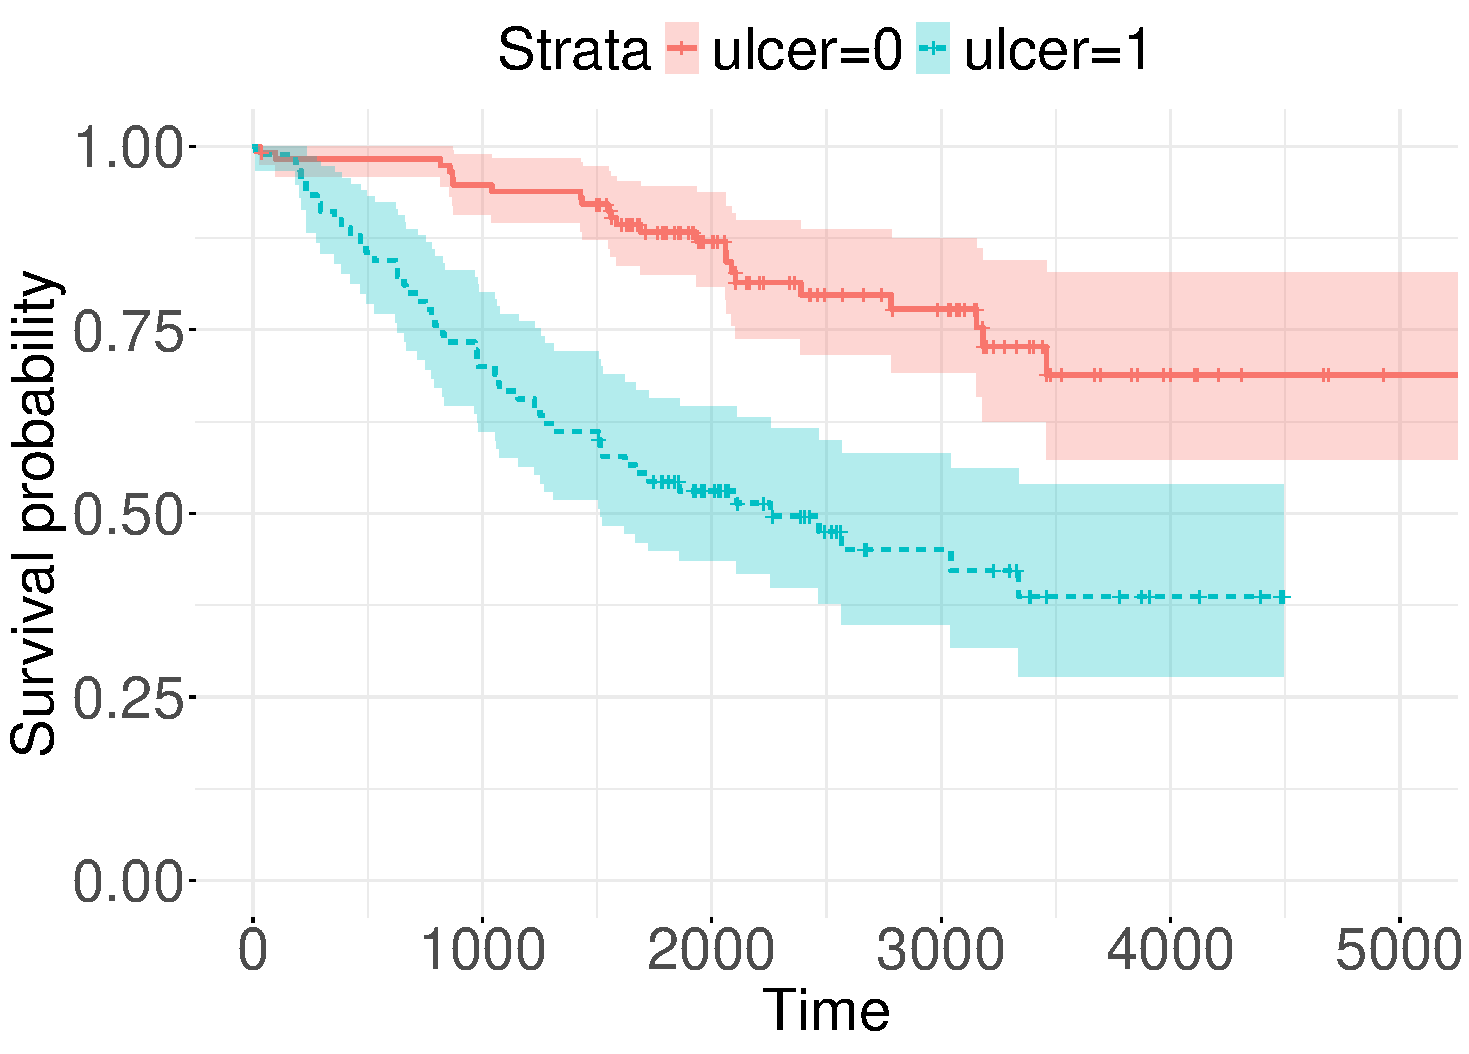
\includegraphics[width = 0.6\textwidth]{figures/KM_plot}
\caption{Sortie du programme R.}
\label{fig:KM_plot}
\end{figure}
Que représente ce graphique? Quels commentaires pouvez vous faire?
\begin{solution}
Le graphique montre les estimateurs de Kaplan-Meier des fonctions de survie des sous-populations dicriminées par la variable \texttt{ulcer}. Les courbes de survies sont bien distinctes. On constate que la présence d'un ulcère augmente la probabilité de décès, la probabilté de survie étant inférieur lorsque $\texttt{ulcer} = 1$.
\end{solution}
\part[2] Nous poursuivons notre analyse avec le programme suivant: 

\begin{lstlisting}
surv_diff <- survdiff(Surv(time, status_os) ~ ulcer, data = melanoma)
surv_diff
\end{lstlisting}

Le résultat est donné par la Figure \ref{fig:survdiff_screen_shot}.

\begin{figure}[!ht]
\centering
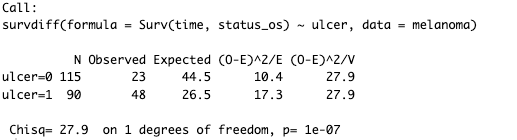
\includegraphics[width = 0.8\textwidth]{figures/survdiff_screen_shot}
\caption{Sortie du programme R.}
\label{fig:survdiff_screen_shot}
\end{figure}

Quelle procédure a-t-on utilisée? Quelle est votre interprétation des résultats?
\begin{solution}
Nous effectuons ici un test du log rang permettant de tester l'hypothèse $H_0$ suivant laquelle les deux courbes de survie sont identiques. La p-valeur conduit à rejeter $H_0$ et à conclure de l'impact significative de la variable \texttt{ulcer} sur la survie des patinets atteints d'un mélanome.
\end{solution}

\part[4] Nous concluons notre étude avec le programme suivant:
\begin{lstlisting}
res.cox <- coxph(
Surv(time, status_os) ~ ulcer + year + age + sex + thickness, 
data = melanoma)
\end{lstlisting}

Le résultat est donné par la Figure \ref{fig:cox_screen_shot}.
\begin{figure}[!ht]
\centering
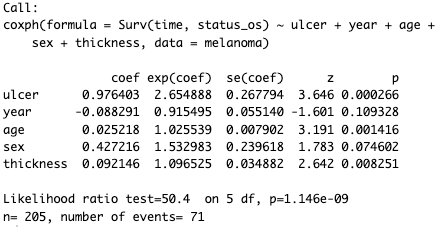
\includegraphics[width = 0.7\textwidth]{figures/cox_screen_shot}
\caption{Sortie du programme R.}
\label{fig:cox_screen_shot}
\end{figure}

Quelle procédure a-t-on utilisée (Rappeler les hypothèses du modèle et l'objectif du modèle)? Quelle est votre interprétation des résultats? 
\begin{solution}
Nous calibrons ici un modèle de hasard proportionnelle qui spécifie la fonction de hasard conditionnellement aux covariables $x$ par 
$$
h(t|x) = h_0(t)e^{\beta x},
$$
où $h_0$ désigne la fonction de hasard de base et le vecteur $\beta$ représente les paramètres du modèle qui caractérise l'impact de chacune des variable sur la fonction de hasard et donc le risque de décès. L'inspection des p-valeur indique que les variable year et sex n'ont pas un impact significatif sur la survie. On observe que la probabilité de décès augmente avec l'âge et la taille de la tumeur. Cette probabilité qugmente également lorsqu'un ulcère est présent. En efet l'exponentielle de ce coefficient est supérieur à $1$ ce qui contribue à augmenter le risque de base.
\end{solution}
\end{parts}
\end{questions}

\end{document}